\chapter{System Design}
In this chapter we will discuss the architecture and design of the \textbf{TechBook} system. In the following sections we will present code snippets and visual diagrams to help portray a basic understanding of the application design. The architecture is modeled on what is known as the MEAN stack and which resembles a three tier architecture. MEAN is a free open-source software stack for building dynamic websites and supports the MVC (Model View Controller) architecture. The contents of this chapter will be seperated into the Data Tier, Logic Tier and Presentation Tier.




\begin{figure}[H]
\begin{minipage}{.4\textwidth}  %listing bloc will have 50% of the line width 
\lstset{linewidth = 4cm, breaklines=true} %set your listing lines widths, and set breaklines to true
\begin{itemize}
\item Database \textbf{MongoDB}
\item Server \textbf{Node.js/express}
\item Client \textbf{Angular.js}
\end{itemize}

\end{minipage}
\qquad %space between listing bloc and the figure
\begin{minipage}{0.6\textwidth} %figure will have the remaning 40% of the line width
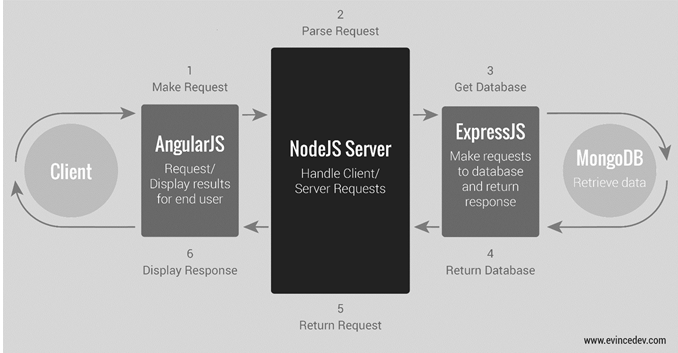
\includegraphics[scale=.4]{img/mvc.png} %the image must be resized or scaled if needed
\caption{MEAN Stack}
\end{minipage}
\end{figure}

% ========================== Databases ========================== 
\section{Database}
For the database adapting the MEAN architecture we used MongoDB.

\subsection{Mongoose}
Harnessing the true power of the Mean stack we used the mongoose object modelling package for Node. Mongoose enabled us to have access to the full suite of MongoDB commands to perform CRUD (Create, Read, Update, Delete) operations. 


To use mongoose we used the following command in the project directory to add it to our Node project:
\begin{minted}{console}
npm install mongoose --save
\end{minted}

Once the package was installed we have to access it in our project :
\begin{lstlisting}[language=JavaScript]
var mongoose = require('mongoose');
\end{lstlisting}

Finally to connect to our MongoDB:
\begin{lstlisting}[language=JavaScript]
// Connect to the mongodb using settings from the config file
mongoose.connect(config.database, { promiseLibrary: require('bluebird') })
  .then(() =>  console.log('\x1b[32m%s\x1b[0m', 'INFO: Connection to database succesfull'))
  .catch((err) => console.error(err));
\end{lstlisting}

\subsection{Mongoose Schema}
Prior to performing CRUD operations we had to define our  mongooses models. These represent documents which can be saved, read and retrieved from our database. The Mongoose Schema is how we define attributes to these documents. To enhance security and the SRP(Single Responsibility Principle) numerous different models were defined and using keys enabled the ability to map relationships to other models.

\begin{figure}[H]
  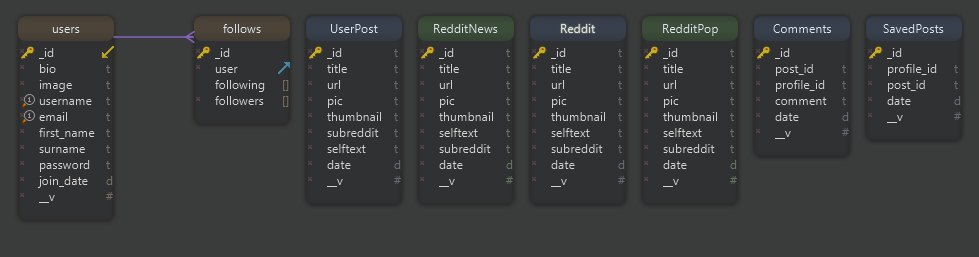
\includegraphics[width=\linewidth]{img/schemas.PNG}
  \caption{MongoDB models}
  \label{fig:schema}
\end{figure}

Figure ~\ref{fig:userscema} below shows how the UserSchema was defined in user.js. The schema was designed to add maximum functionality while also protecting the system from having invalid objects added to the database. There are a few things to note about this particular schema.
\begin{itemize}
\item \textbf{Uniqueness} : The \textit{username} and \textit{email} fields are set to unique. This ensures a user can only have one account per email and that the username will not not cause issues when a search query is performed.
\item \textbf{Required} : The \textit{username}, \textit{firstname},\textit{surname} and \textit{password} fields are required. These represent the bare minimum that must be initialised to have a valid account.
\item \textbf{Default} : The \textit{joindate},\textit{bio} and \textit{image} are set to default. This allows a faster user registration with a default image used, the join date set to the current date and a generic bio that can all be updated using the settings link.
\end{itemize}

\begin{lstlisting}[language=JavaScript,caption={Defining User Schema},captionpos=b,label={fig:userscema}]
// Schema used to 'filter' data to be stored in the 'UserSchema' collection in mongo
var UserSchema = new mongoose.Schema({
  username: {
    type: String,
    unique: true,
    required: true
  },
  email: {
    type: String,
    unique: true,
  },
  first_name: {
    type: String,
    required: true
  },
  surname: {
    type: String,
    required: true
  },
  join_date: {
    type: Date,
    default: Date.now
  },
  bio: {
    type: String,
    default: 'Tell me about yourself'
  },
  image:{
    type: String,
    default: 'profile.jpg'
  },
  password: {
    type: String,
    required: true
  }
});

\end{lstlisting}

\subsection{Password hashing}
To ensure the highest standard of security any confidential user information should never directly be stored in a database. Mongoose allows us to define functions using 'pre(function,functionToExecute)' that executes prior to saving a document. Bcrypt a node-module that simplifies hashing can be used to both encrypt and decrypt sensitive data. Combining the use of these technologies when a user account is created or modified, the password is hashed before saving the document and in turn the hashed value of the password is saved in the database thus protecting the origonal password being exposed in the event of a malicious attack.

\begin{lstlisting}[language=JavaScript,caption={Password Hashing},captionpos=b,label={fig:presave}]
// define pre hook for document
UserSchema.pre('save', function (next) {
  var user = this;
  // if password new or edited
  if (this.isModified('password') || this.isNew) {
    // generate a salt and process data for 10 rounds
    bcrypt.genSalt(10, function (err, salt) {
      if (err) {
        return next(err);
      }
      // generate a hash of password
      bcrypt.hash(user.password, salt, null, function (err, hash) {
        if (err) {
          return next(err);
        }
        user.password = hash;
        next();
      });
    });
  } else {
    return next();
  }
});

\end{lstlisting}
Ensuring the password is hashed is of major importance but equally as crucial is the ability to be able to compare the hashed value with a password entered by a user attempting to log in. To achieve this we were able to attach a comparePassword function to the UserSchema which executes the compare method from the bcrypt module and checks for a match between the password entered and the hashed password stored in the database as shown in Figure ~\ref{fig:passcheck}. 
\begin{lstlisting}[language=JavaScript,caption={Password Comparision},captionpos=b,label={fig:passcheck}]
// compare password for log in
UserSchema.methods.comparePassword = function (passw, cb) {
  bcrypt.compare(passw, this.password, function (err, isMatch) {
    if (err) {
      return cb(err);
    }
    cb(null, isMatch);
  });
};
\end{lstlisting}

\subsection{JSON Web tokens}
% ========================== Authentication ========================== 
\section{Authentication}
What database like

% ========================== API Calls ========================== 
\section{API/HTTP}
How we designed api calls/
insert info from swagger

% ========================== UI ========================== 
\section{Client UI}
The presentation tier is based on the Angular front-end web framework. In contrast to traditional multiple page web applications the Client is presented as a single page application in which components are injected into. In this section we will look at the Angular app structure, the services which allow us to interact with our node js server and the finished view of the pages.

\subsection{Angular folder structure}

\subsection{Angular Services}
The Angular services allow our application to interact and access data from our database via the node server. Thus keeping data retrieval separate to page functions. In the services we provide the logic to process HTTP requests to the API to perform CRUD operations on the data served by the Node.js/ExpressJS server. 

\subsection{Page views}
In this section we will look at some screen shots of the web application from the view of a PC web browser and on a Samsung Galaxy S6 mobile device. For each page a brief summary of the functionality of the page will be provided along with any input validation that was used. 
How we designed the ui
few screenshots off finished site


\subsubsection{Navigation Pane}
The header component is injected into the main index.js view. This allows us to render the navigation pane at all times while the main content view is adapted to the selected page view. The header component contains a header logo displaying the image that was designed for the application and a navigation bar with numerous features. When designing the navbar we decided it must meet the following conditions: appealing, easy to use and fully functional, all whilst being fully responsive to changing screen sizes and different devices.

To add the the functionality when a user enters the site and is not currently logged in the navbar contains a log in form that enables a user to log in. As long as a user is not logged in all other functionality from the navbar is disabled as seen in Figure ~\ref{fig:header} . To add to the pleasing aesthetic the navbar is also made sticky. Figure ~\ref{fig:headerStick} shows that when the page is scrolled down the header logo will scroll out of view and the navbar will stay located at the top of the page.

\begin{figure}[H]
\centering
\begin{minipage}{.5\textwidth}
  \centering
  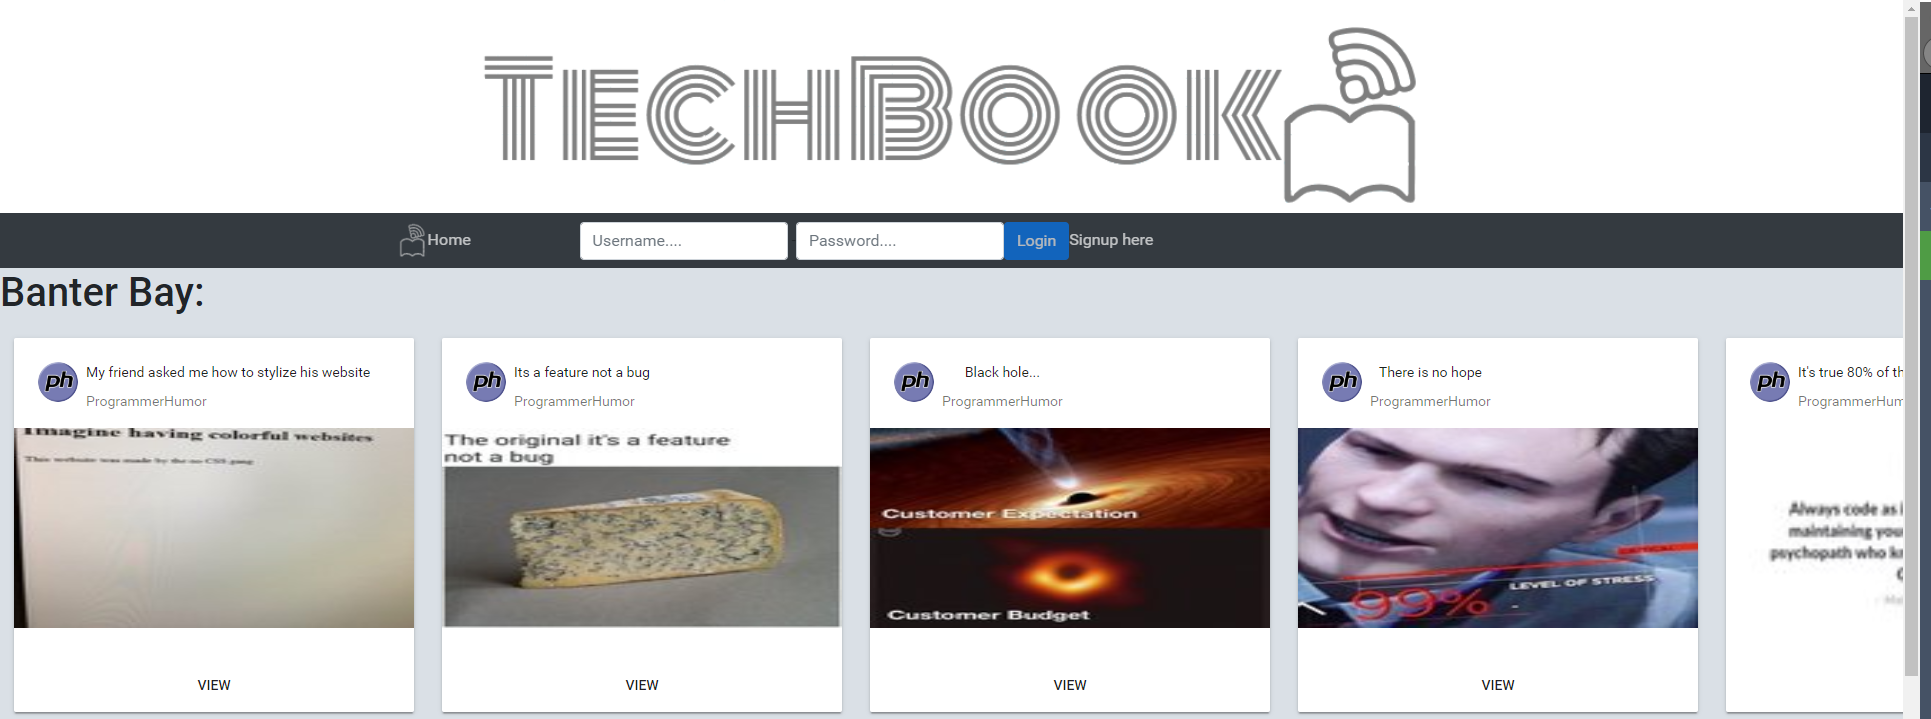
\includegraphics[width=.9\linewidth]{img/ui/headerPC.PNG}
  \captionof{figure}{Header}
  \label{fig:header}
\end{minipage}%
\begin{minipage}{.5\textwidth}
  \centering
  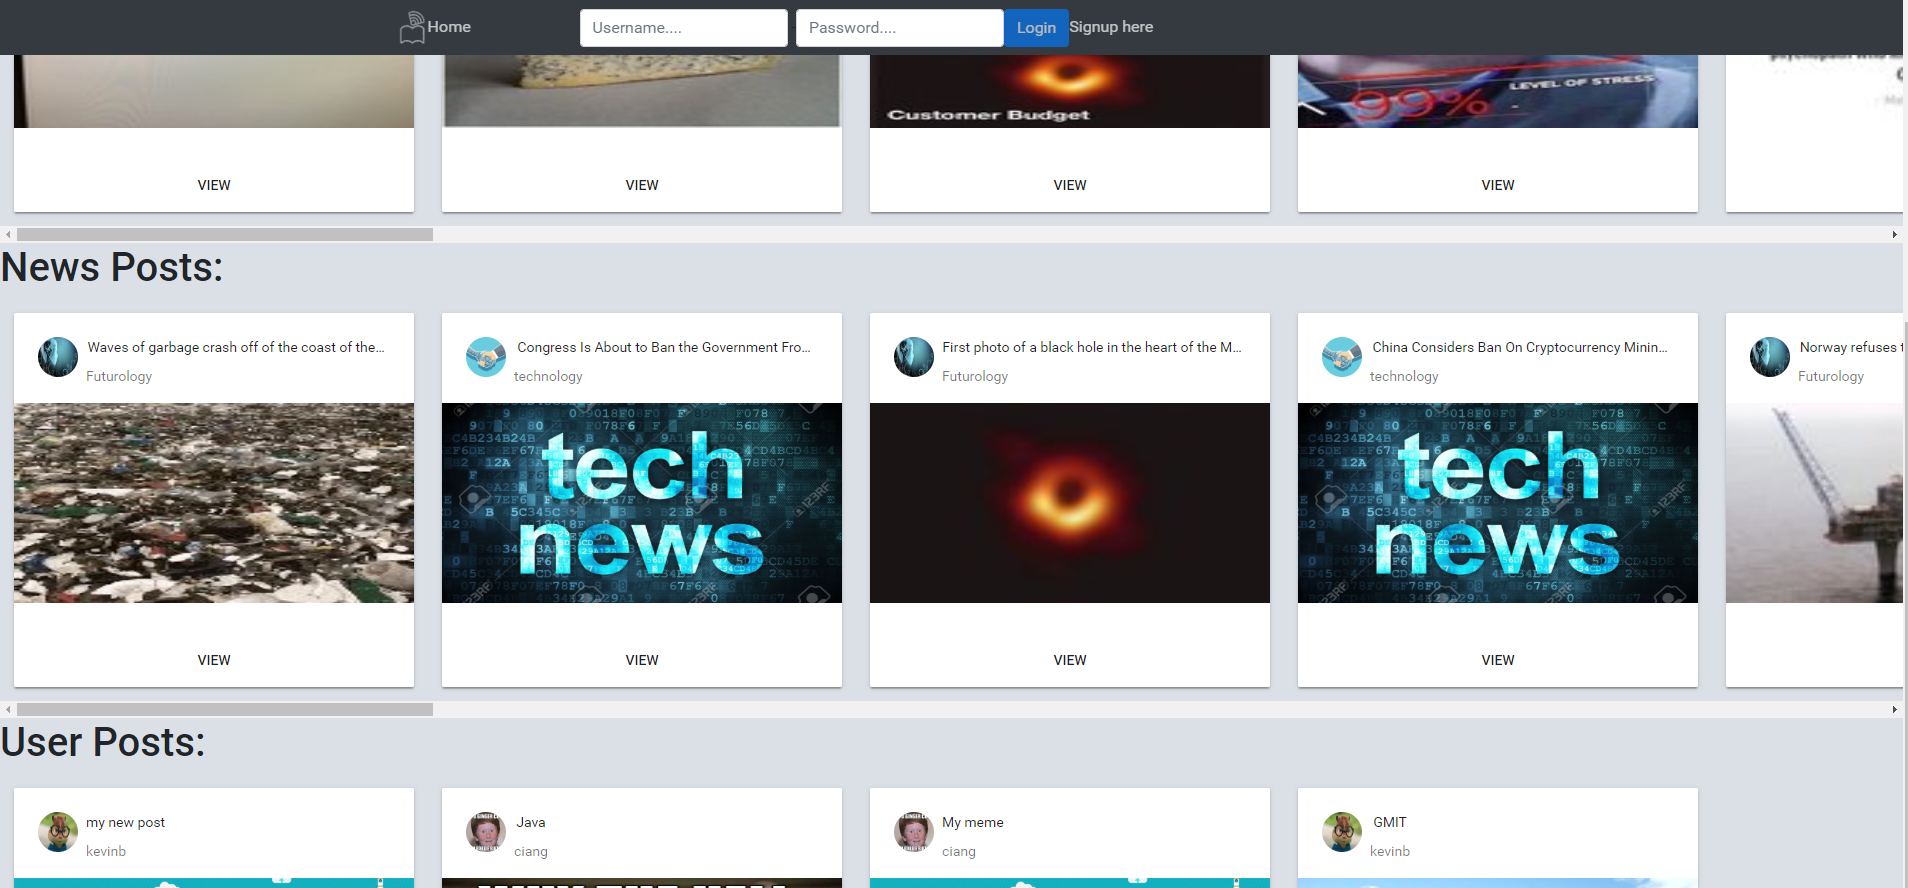
\includegraphics[width=.9\linewidth]{img/ui/headerpcsticky.PNG}
  \captionof{figure}{Sticky Navbar}
  \label{fig:headerStick}
\end{minipage}
\end{figure}

However when the user is logged in even more functionality is active. Shown in Figure  ~\ref{fig:headernodrop} relating general site functions three buttons with corresponding icons are added to redirect the user to the the Home, Make Post and About Us page. For functions related to the current user, a drop down menu was added along with the logged in users thumbnail photo and username. Selecting the arrow icon displayed in Figure\ref{fig:headerdrop} displays a drop down menu. This menu has options to render the Profile, Account Settings, Friends and Saved post pages. The Logout button in the drop down menu logs the user out, deletes the JWT token from session storage and redirects to the homepage. 
\begin{figure}[H]
\centering
\begin{minipage}{.5\textwidth}
  \centering
  
\includegraphics[width=.9\linewidth]{img/ui/headernodrop.PNG}
  \captionof{figure}{Navbar}
  \label{fig:headernodrop}
\end{minipage}%
\begin{minipage}{.5\textwidth}
  \centering
  
\includegraphics[width=.9\linewidth]{img/ui/headerdrop.PNG}
  \captionof{figure}{Navbar Dropdown active}
  \label{fig:headerdrop}
\end{minipage}
\end{figure}



\subsubsection{Log in Page}
The log in page consists of of a username and password input box. In order to submit a login attempt both values must be supplied. The values are then authenticated on the server and if successful the server returns a JWT token that's stored in session storage and the user is redirected to the homepage view.  If the username is invalid the server will return a "Log in failed. User not found." error message to the view or in the case of an invalid password a "Incorrect password" message is returned.
\begin{figure}[H]
\centering
\begin{minipage}{.75\textwidth}
  \centering
  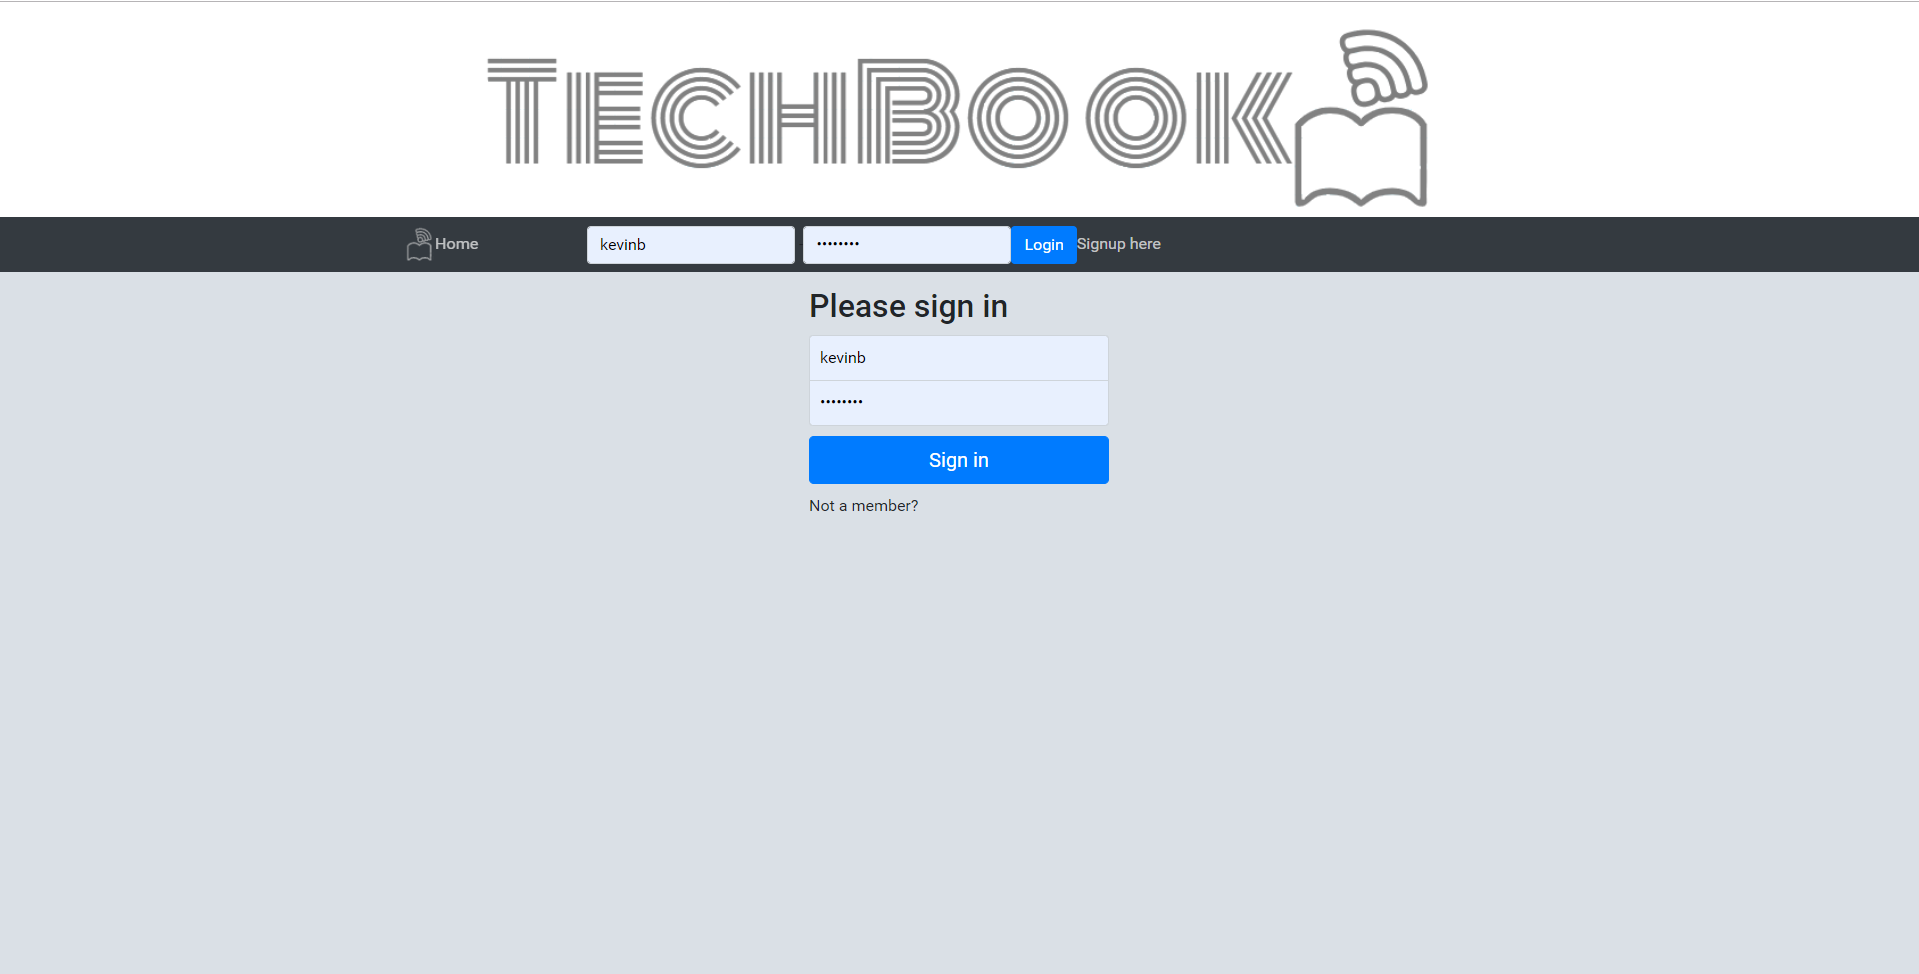
\includegraphics[width=.9\linewidth]{img/ui/login_PC.PNG}
  \captionof{figure}{Web View}
  \label{fig:loginPC}
\end{minipage}%
\begin{minipage}{.25\textwidth}
  \centering
  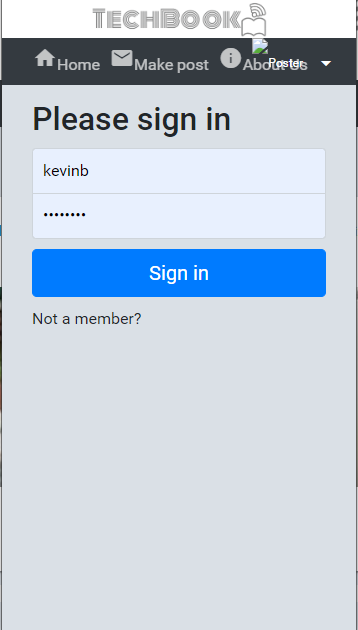
\includegraphics[width=.9\linewidth]{img/ui/login_MOBILE.PNG}
  \captionof{figure}{Mobile view}
  \label{fig:loginMOBILE}
\end{minipage}
\end{figure}

\subsubsection{Register Page}
The register page allows a user to enter credentials for a new user profile. To submit a register attempt all fields are required. This page view contains numerous different aspects that must be validated:


\begin{figure}[H]
\begin{minipage}{.5\textwidth}  %listing bloc will have 50% of the line width 
\lstset{0.6\textwidth, breaklines=true} %set your listing lines widths, and set breaklines to true
\begin{itemize}
\item Username : Required, Must be unique to server.
\item firstname : Required.
\item surname : Required.
\item email : Required, Must contain '@' followed by '.' symbol, Must be unique to server.
\item Password : Must be 8 characters and must match confirm password value.
\end{itemize}

\end{minipage}
\qquad %space between listing bloc and the figure
\begin{minipage}{0.4\textwidth} %figure will have the remaning 40% of the line width
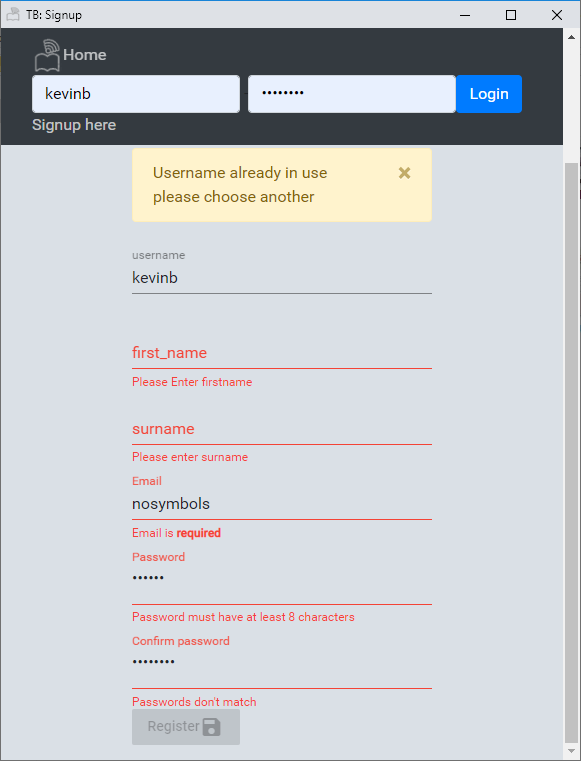
\includegraphics[width=.9\linewidth]{img/ui/signuperror.PNG} %the image must be resized or scaled if needed
\caption{Register Validation}
\end{minipage}
\end{figure}

\begin{figure}[H]
\centering
\begin{minipage}{.75\textwidth}
  \centering
  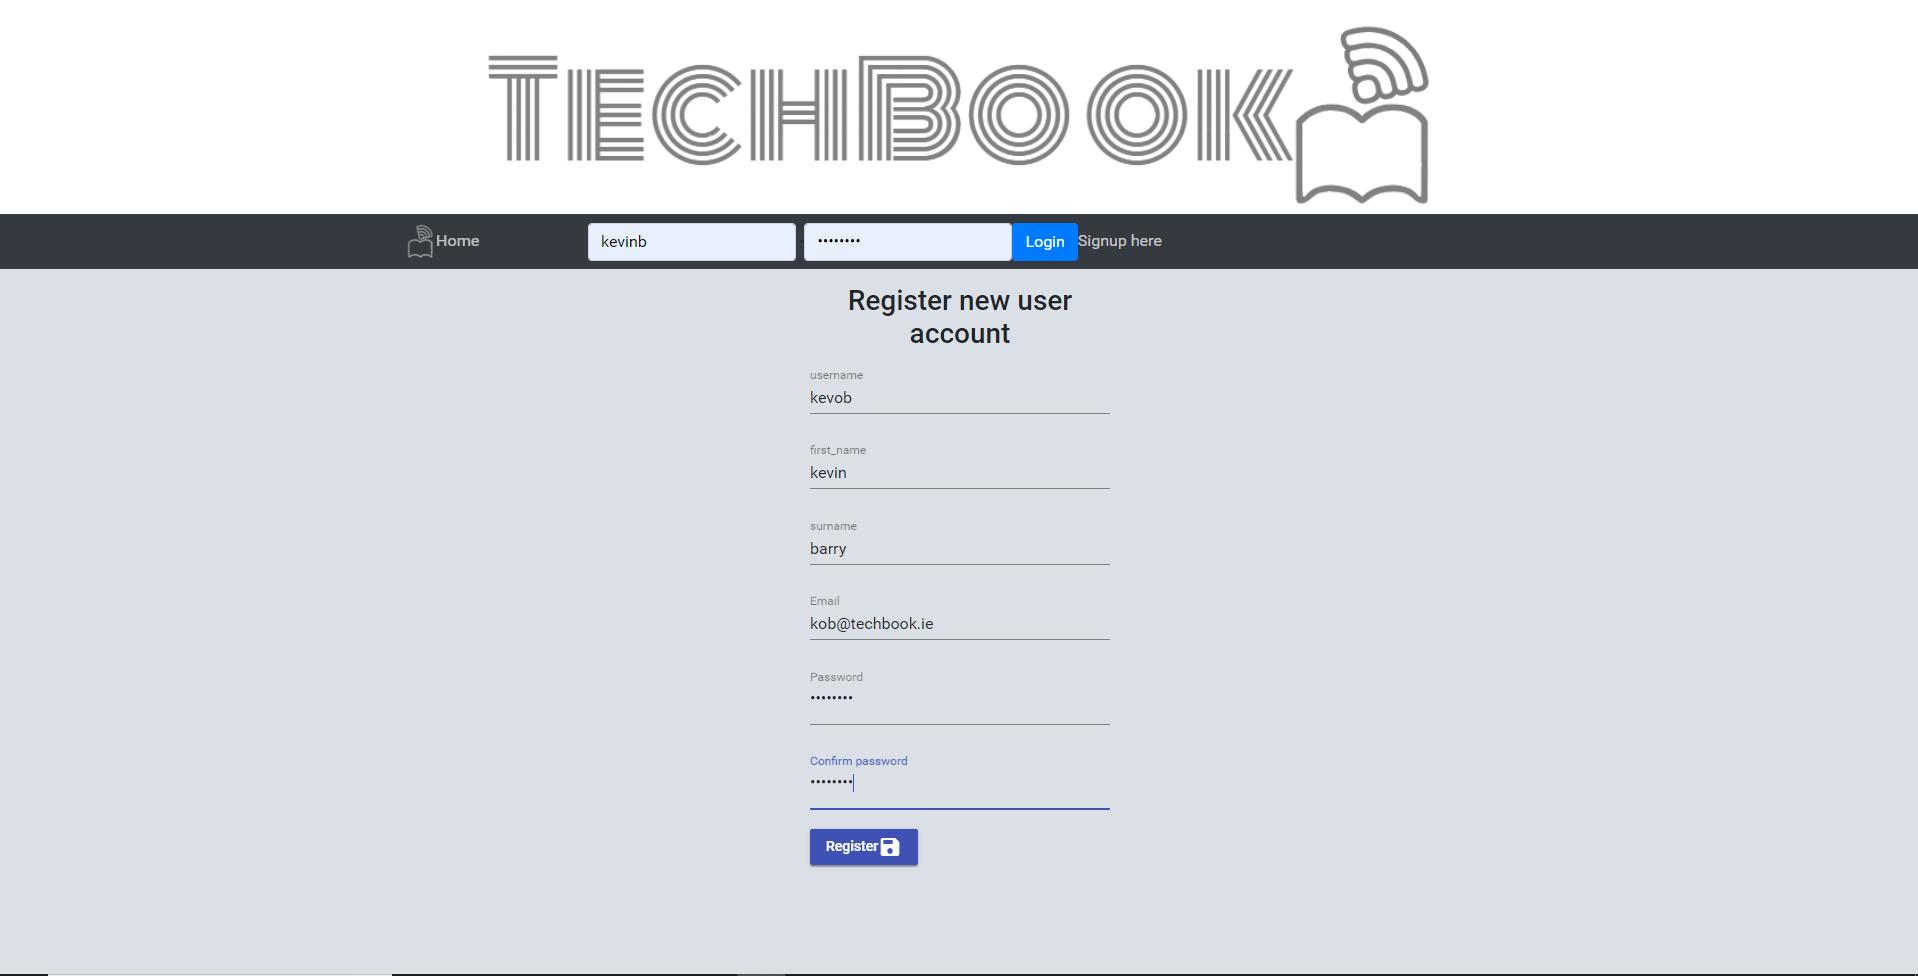
\includegraphics[width=.9\linewidth]{img/ui/sigup_PC.PNG}
  \captionof{figure}{Web View}
  \label{fig:signupPC}
\end{minipage}%
\begin{minipage}{.25\textwidth}
  \centering
  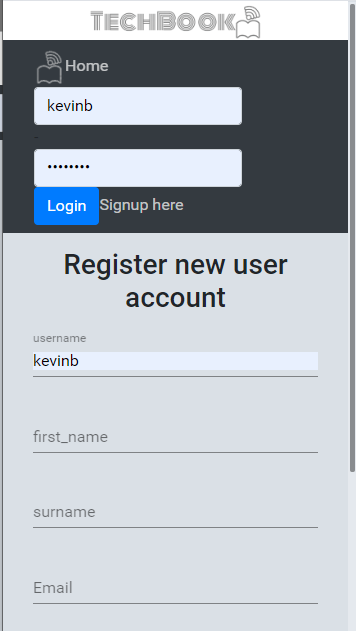
\includegraphics[width=.9\linewidth]{img/ui/signup_MOBILE.PNG}
  \captionof{figure}{Mobile view}
  \label{fig:signupMOBILE}
\end{minipage}
\end{figure}

\subsubsection{Profile Page}
\begin{figure}[H]
\centering
\begin{minipage}{.75\textwidth}
  \centering
  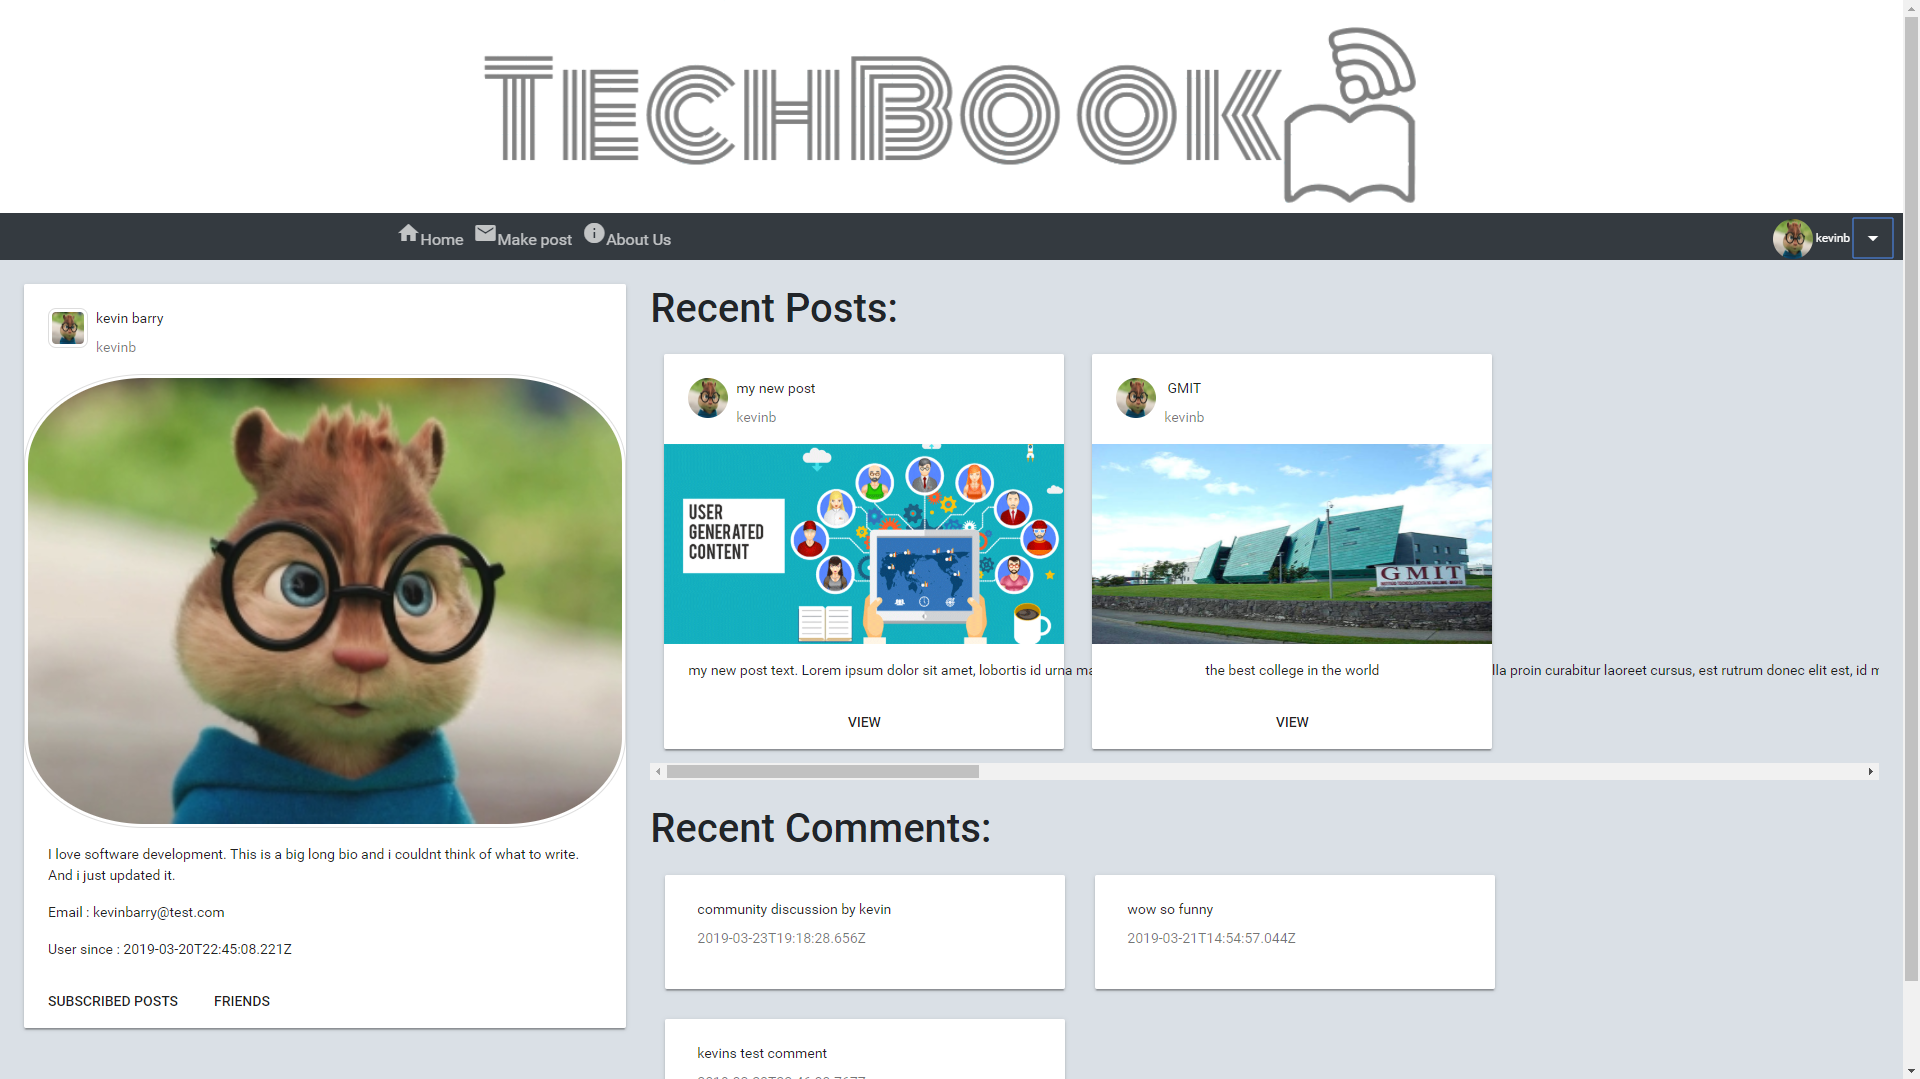
\includegraphics[width=.9\linewidth]{img/ui/profile_PC.PNG}
  \captionof{figure}{Web View}
  \label{fig:profilePC}
\end{minipage}%
\begin{minipage}{.25\textwidth}
  \centering
  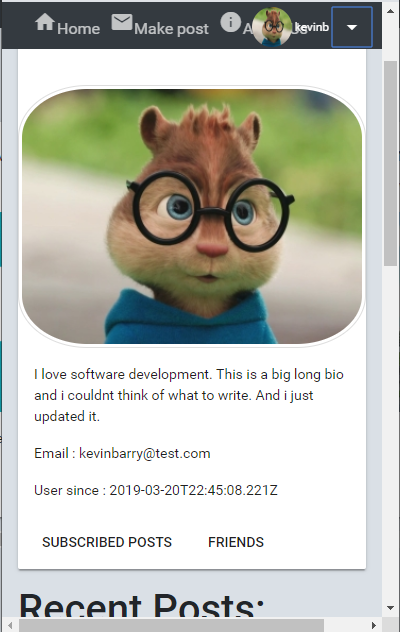
\includegraphics[width=.9\linewidth]{img/ui/profile_MOBILE.PNG}
  \captionof{figure}{Mobile view}
  \label{fig:profileMOBILE}
\end{minipage}
\end{figure}

\subsubsection{Settings Page}
The settings page view allows a user to edit their current credentials and is accessed by clicking the settings tab on the navbar drop down menu. The form fields are pre-filled from the users data retrieved by the server.

\begin{lstlisting}[language=JavaScript,caption={Auto fill form data},captionpos=b,label={fig:userscema}]
/**
 * Set the form data in SettingsForm to the details of the current user.
 * 
 * @param id The current users id.
 */
setForm(id) {
  this.userService.getProfile(id)
    .subscribe(profile => {
      // Must extract profile data from response.
      this.profileinfo = profile[0];
      // Form object
      this.settingsForm.setValue({
        email: this.profileinfo.email,
        first_name: this.profileinfo.first_name,
        surname: this.profileinfo.surname,
        bio: this.profileinfo.bio
      });
    });
}
\end{lstlisting}
 This page also allows the user to update or change their current profile image. Selecting the 'choose file' button pops up a file explorer window and allows the user to select an image. The chosen image is then shown in a preview tab so the user can have a peek prior to selecting the "Upload new profile image" button. This was achieved by importing the \textbf{ng2-file-upload} module and applying custom functions. The uploaded image is then saved in a image folder on the server and the users account is updated with the location to access this image. The uploader is also validated to only accept image files.
\begin{figure}[H]
\centering
\begin{minipage}{.75\textwidth}
  \centering
  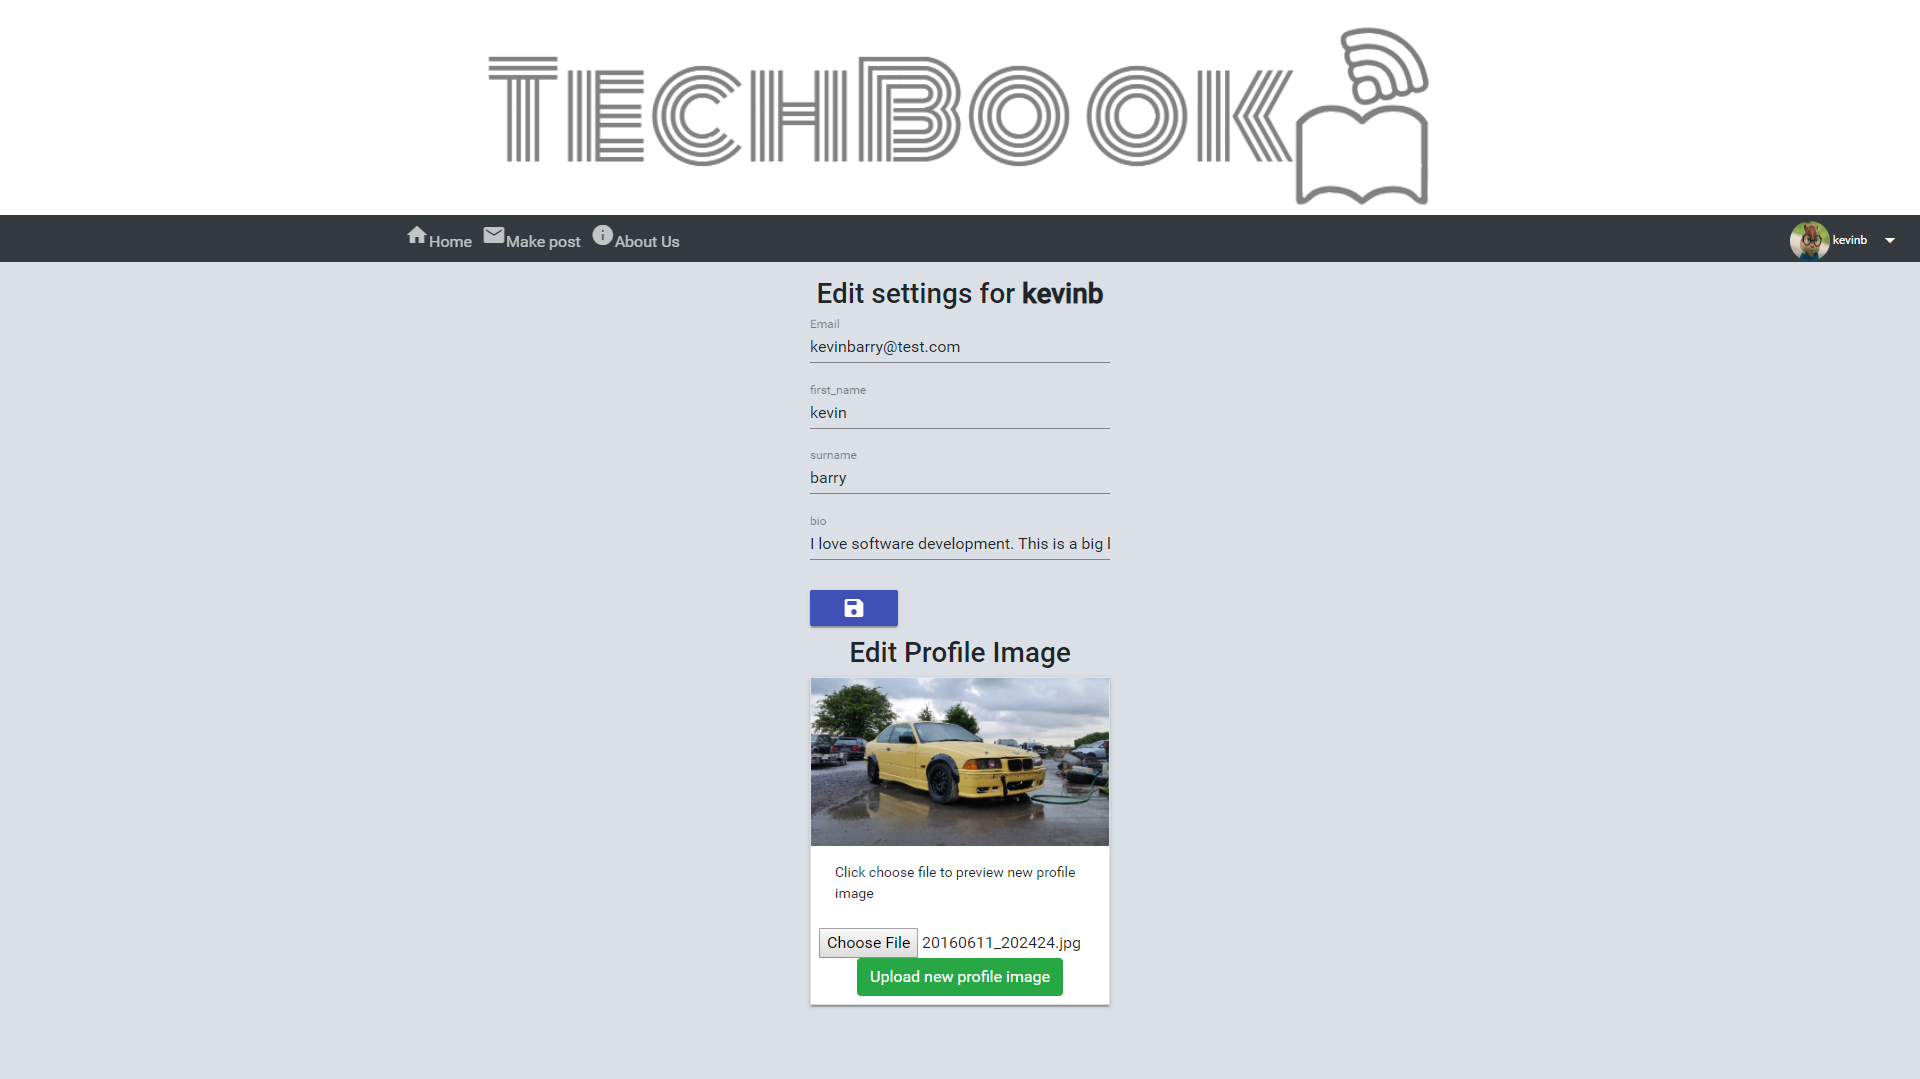
\includegraphics[width=.9\linewidth]{img/ui/settings_PC.PNG}
  \captionof{figure}{Web View}
  \label{fig:settingsPC}
\end{minipage}%
\begin{minipage}{.25\textwidth}
  \centering
  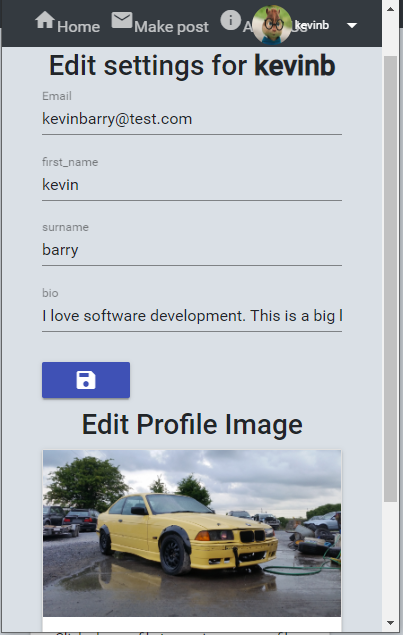
\includegraphics[width=.9\linewidth]{img/ui/settings_MOBILE.PNG}
  \captionof{figure}{Mobile view}
  \label{fig:settingsMOBILE}
\end{minipage}
\end{figure}

\subsubsection{Friends Page} 
The friends page is a view that allows a user to toggle a view between followers and following. This page can be accessed in two ways which render different views. If a user wants to view a list of their own followers and who they are following they can select the "Friends" button in the navbar drop down menu. If a user would like to view another users followers and following list a button "Follows" can be selected on the preferred users profile page. The lists contain cards that show a image avatar, username and bio for each user. To view a users profile from this view simply click on the username and the system redirects you to that users profile page.
\begin{figure}[H]
\centering
\begin{minipage}{.75\textwidth}
  \centering
  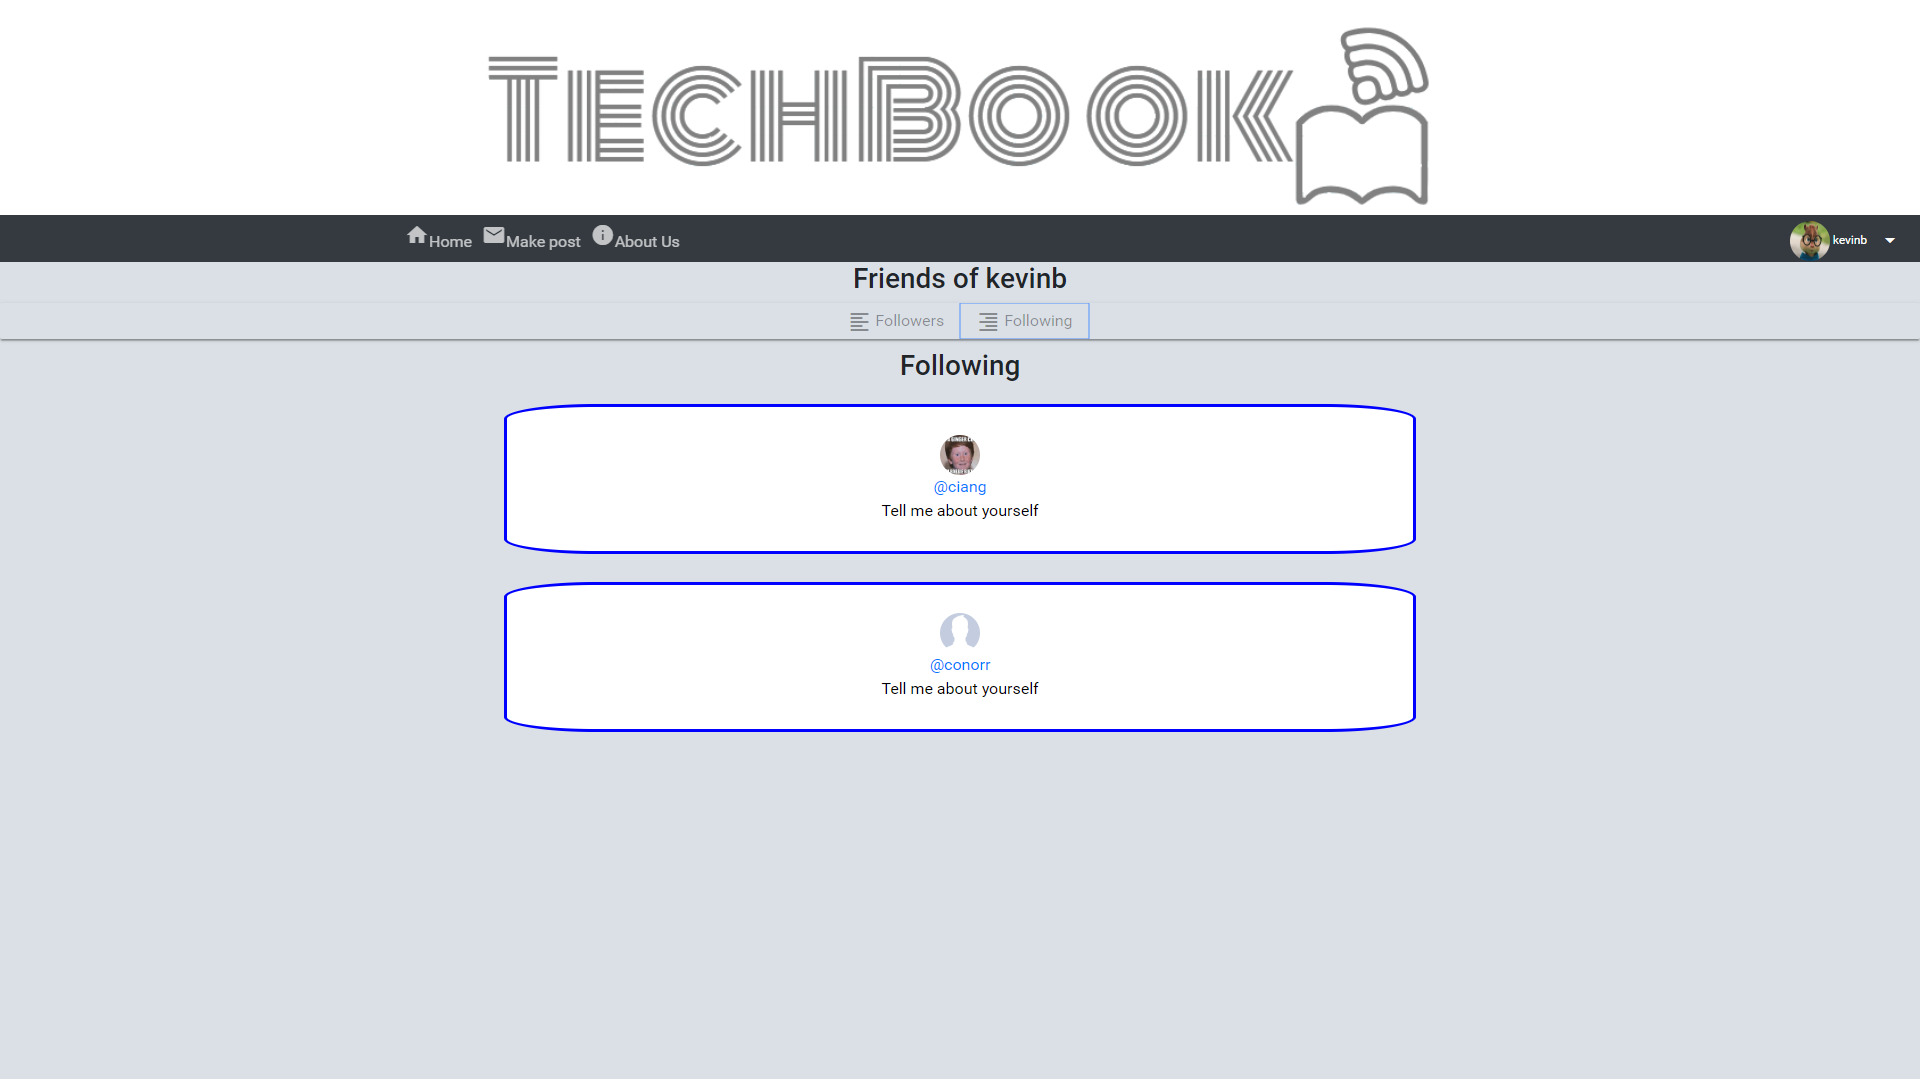
\includegraphics[width=.9\linewidth]{img/ui/followPC.PNG}
  \captionof{figure}{Web View}
  \label{fig:followPC}
\end{minipage}%
\begin{minipage}{.25\textwidth}
  \centering
  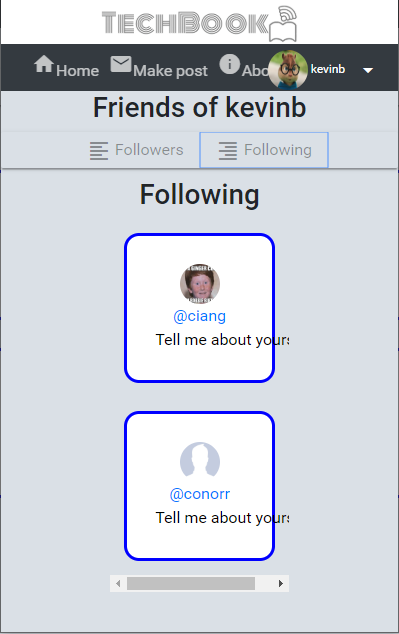
\includegraphics[width=.9\linewidth]{img/ui/followMOBILE.PNG}
  \captionof{figure}{Mobile view}
  \label{fig:followMOBILE}
\end{minipage}
\end{figure}

\subsubsection{Home Page}

\begin{figure}[H]
\centering
\begin{minipage}{.75\textwidth}
  \centering
  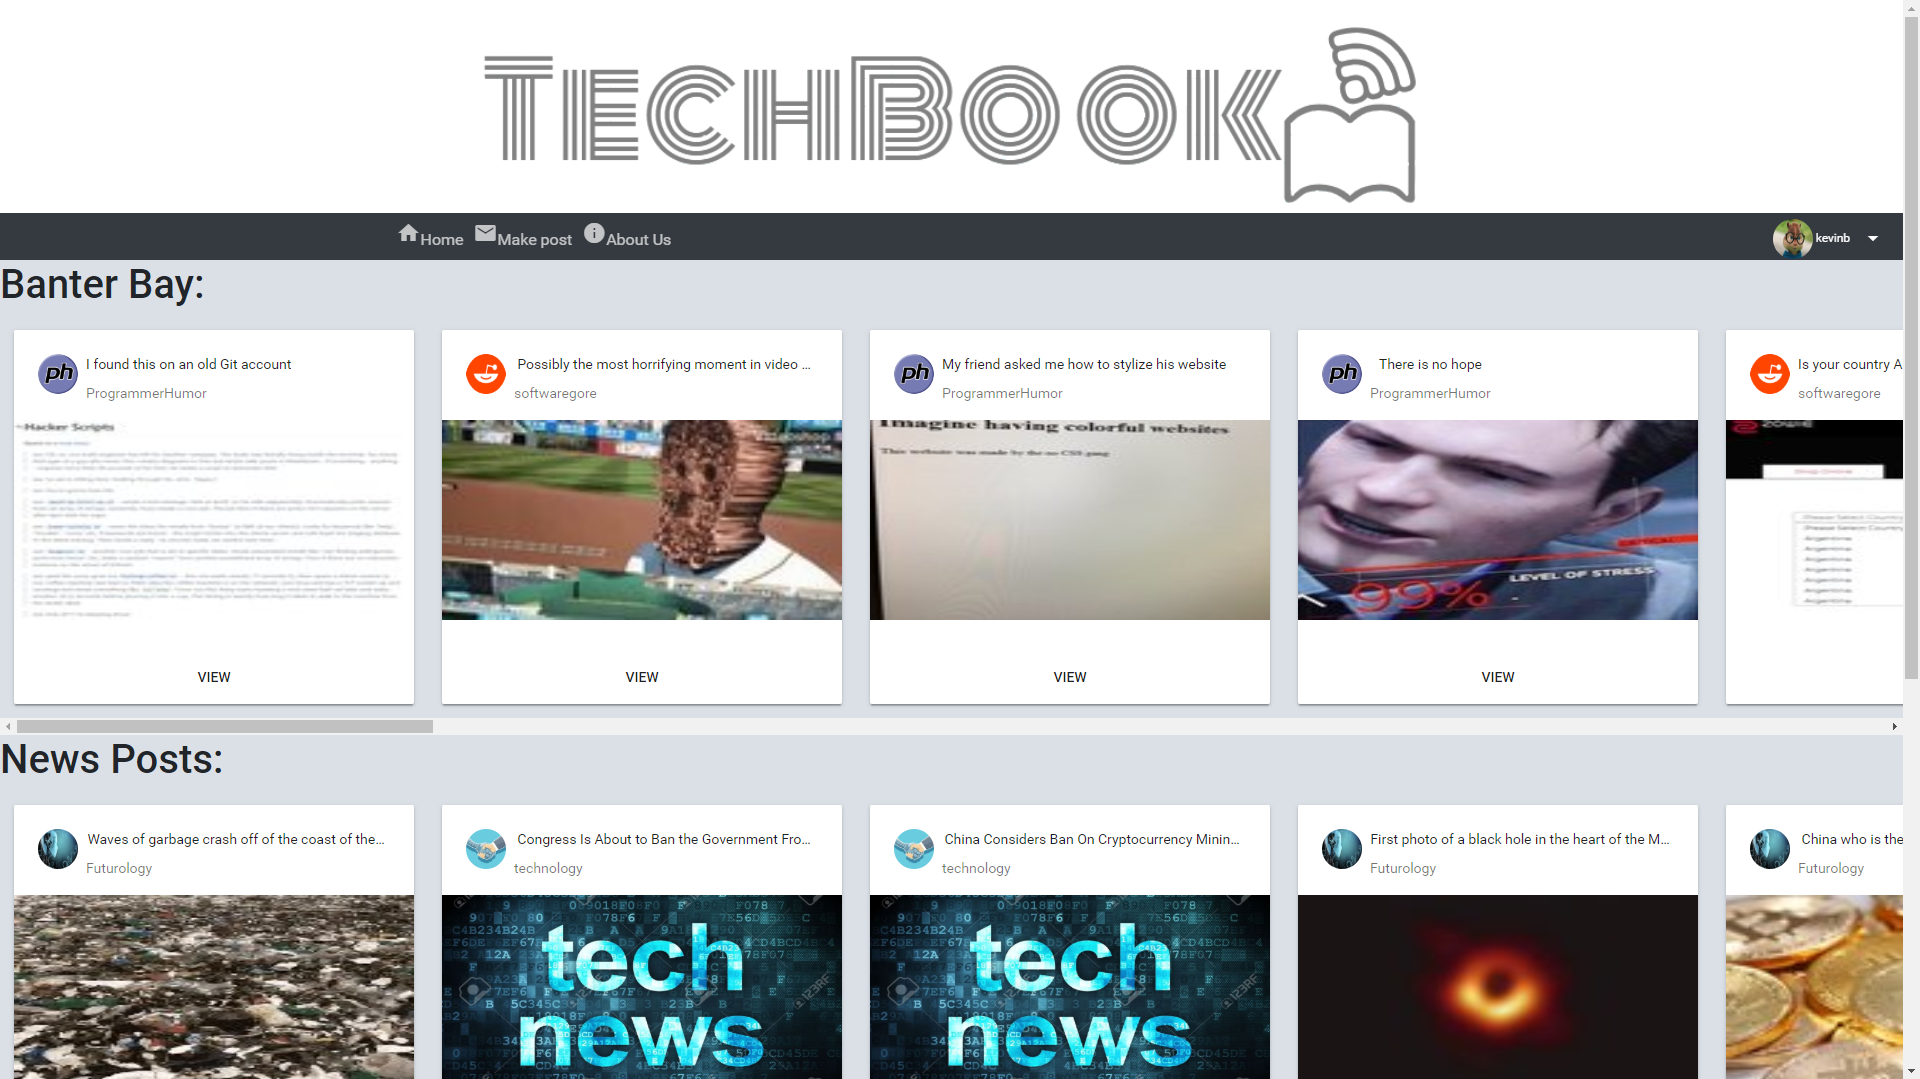
\includegraphics[width=.9\linewidth]{img/ui/homepcsnap.PNG}
  \captionof{figure}{Web View}
  \label{fig:test1}
\end{minipage}%
\begin{minipage}{.25\textwidth}
  \centering
  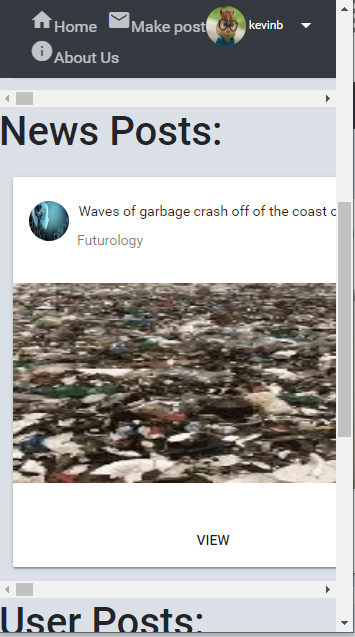
\includegraphics[width=.9\linewidth]{img/ui/homemobile.PNG}
  \captionof{figure}{Mobile view}
  \label{fig:test2}
\end{minipage}
\end{figure}

\subsubsection{Posts Page}
\subsubsection{About Page}
The purpose of the about page view is to give the user an insight into the project. The view is separated into three sections with each item being displayed on its own card. Each card consists of an image, a link to the resource, a summary of the resource link and also some brief information on that item. The Team section is a over view of the developers of the web application with clickable link to view our Github profiles. The Documentation section contains links to the project source code, dissertation and the Swagger documentation for the API. The third section is used to provide links to resources and give information on some of the components used in the project such as  MEAN Stack, MongoDB, Express.js, Angular, Node.JS, Reddit API, Passport.JS, HTML and CSS.
\begin{figure}[H]
\centering
\begin{minipage}{.75\textwidth}
  \centering
  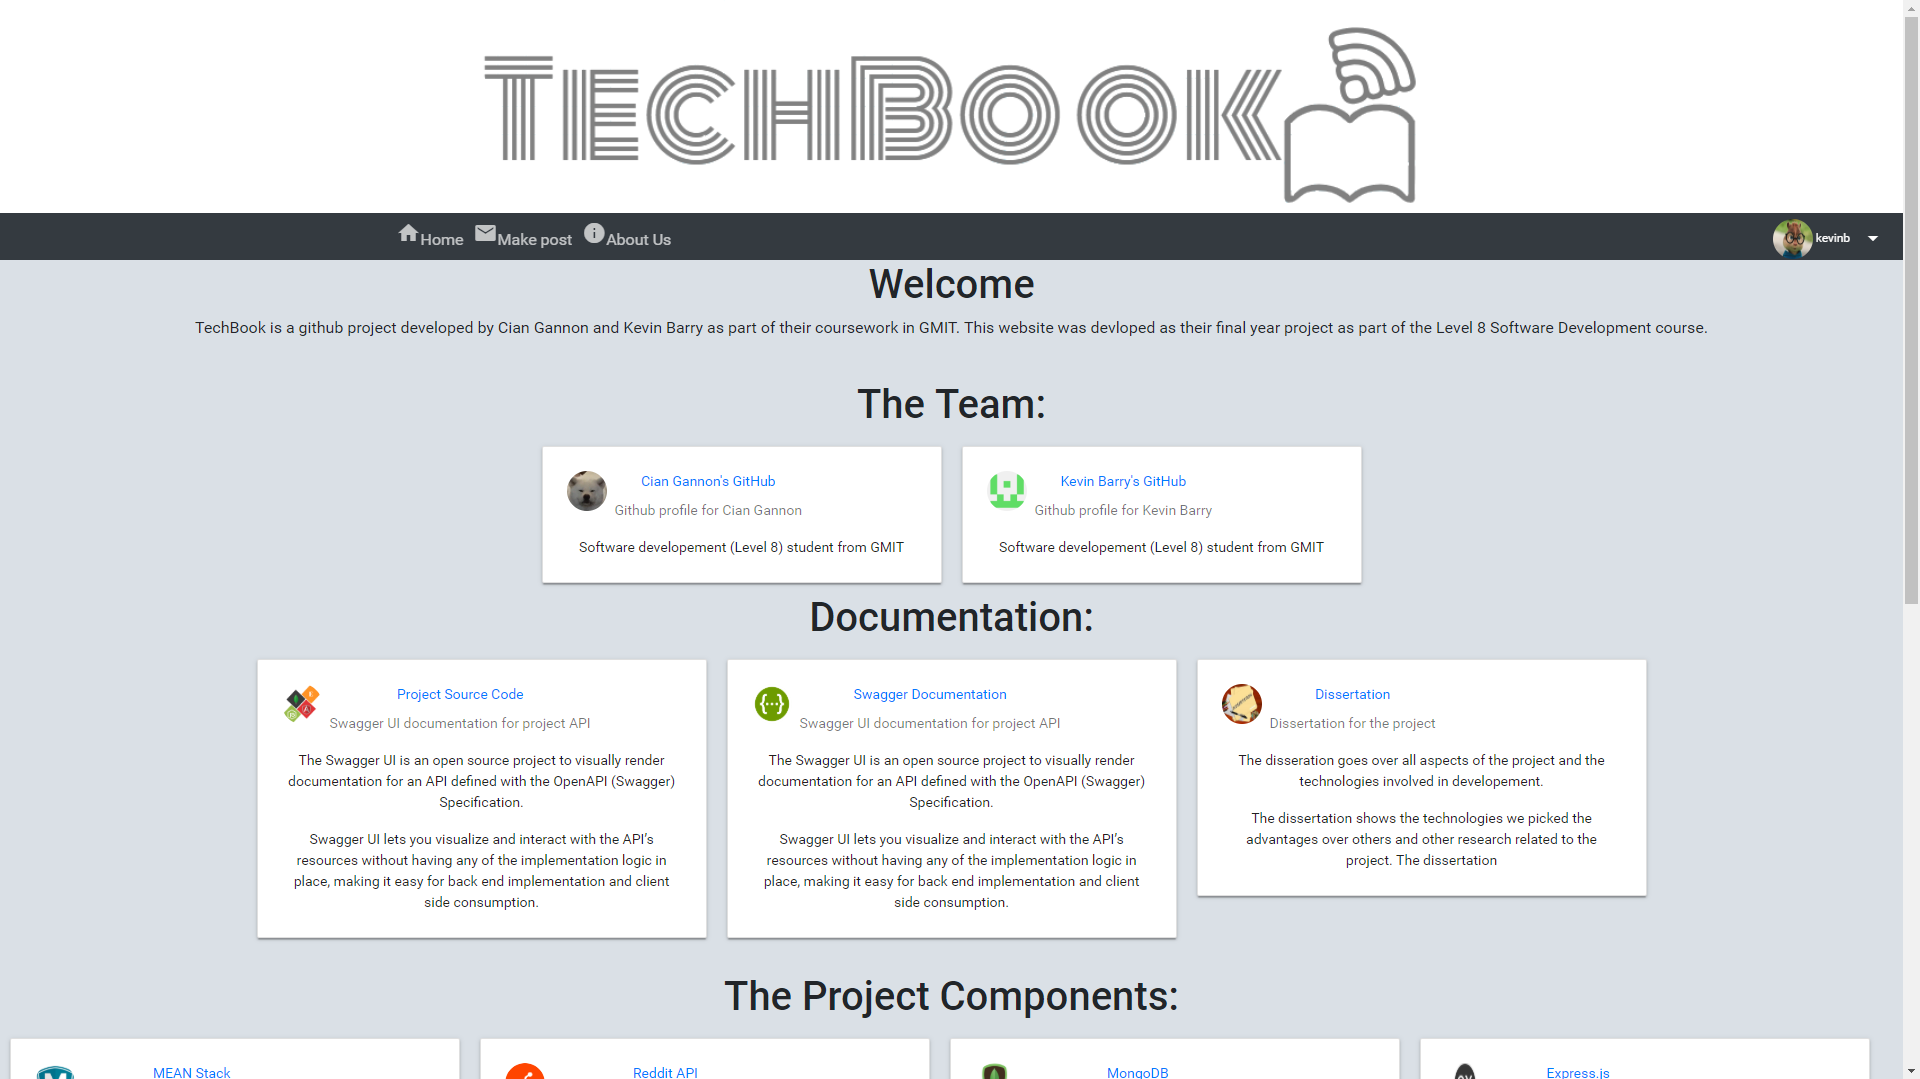
\includegraphics[width=.9\linewidth]{img/ui/about_PC.PNG}
  \captionof{figure}{Web View}
  \label{fig:aboutPC}
\end{minipage}%
\begin{minipage}{.25\textwidth}
  \centering
  
\includegraphics[width=.9\linewidth]{img/ui/about_MOBILE.PNG}
  \captionof{figure}{Mobile view}
  \label{fig:aboutMobile}
\end{minipage}
\end{figure}
\begin{itemize}
\item Architecture, UML etc. An overview of the different components of the system. Diagrams etc… Screen shots etc.
\end{itemize}

\begin{table}[h]
  \centering
  \begin{tabular}{x{2cm}p{3cm}}
    \toprule \\
    Column 1 & Column 2 \\
    \midrule \\
    Rows 2.1 & Row 2.2 \\
    \bottomrule
  \end{tabular}
  \caption{A table.}
  \label{table:mytable}
\end{table}